%! Author = Tom
%! Date = 07.12.2022
\chapter{Einleitung}

In diesem Kapitel wird an das Thema herangeführt und die Motive dargestellt.
Es wird definiert, welche Ziele in dieser Arbeit verfolgt werden.
Abschließend folgt eine Übersicht über die Kapitelstruktur.

\section{Motivation}

Mit einer steigenden Nutzung von GraphQL wird es immer wichtiger, Tests für GraphQL-Schnittstellen zu entwickeln, damit eine gute Softwarequalität sichergestellt werden kann.
Die Entwicklung von Tests kann manuell oder automatisch geschehen.
Bei Unit-Tests, also Tests für einzelne Funktionen, kann ein Programmierer selbst entscheiden, ob er diese manuell erstellt
oder von einem Tool automatisch generieren lassen will.
Integrations-Tests, also Tests, die Kombinationen von Interaktionen in Modulen miteinander testen, hingegen haben sehr oft
einen sehr großen Testraum, sodass ein manuelles Erstellen dieser Tests fehleranfällig und langwierig ist.
Im Folgenden wird der Begriff API öfters genutzt werden, die Klärung des Begriffs findet sich in Kapitel~\ref{api}.
Für REST-APIs existieren schon automatische Integrationstesttools wie zum Beispiel: EvoMaster~\cite{evo-master}, QuickREST~\cite{karlsson2019quickrest} oder RESTTESTGEN~\cite{rest-test-gen}.
GraphQL-APIs haben leider noch einen Mangel an solchen automatischen Testtools.
Im Rahmen der internationalen  Konferenz für Automatisierung  von  Softwaretests IEEE/ACM 2021 wurde mit
\textit{Automatic Property-based Testing of GraphQL APIs}~\cite{property-based-testing} eine Methode vorgestellt, die diesen Mangel angehen soll.
Es wurde eine Methode entwickelt, die aus dem GraphQL-Schema, also der Beschreibung der Datenstruktur der API, Tests zufällig generiert und damit versucht, Fehler in der Programmierung zu finden.
Die entwickelte Methode arbeitet nach dem in Abbildung~\ref{property-based-method} gezeigten Prinzip.

\begin{figure}[h!]
    \centering
    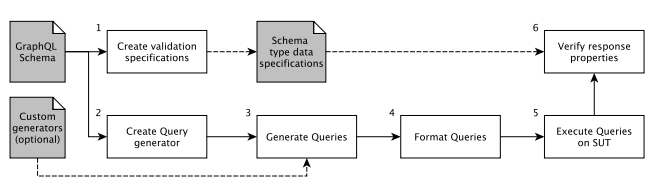
\includegraphics[width=\textwidth,height=\textheight,keepaspectratio]{content/einleitung/toolchain}
    \caption{Methode von~\cite{property-based-testing}}
    \label{property-based-method}
\end{figure}
\newpage

Es wird aus einem GraphQL-Schema ein Testgenerator entwickelt.
Dieser kann aus der Typspezifikation, die GraphQL vorgibt, valide GraphQL-Querys entwickeln und diese mit verschiedenen Argumenten anreichern.
Die generierten Querys stellen die entwickelten Tests dar.
Das Besondere an GraphQL ist jedoch, dass es einen Graphen umsetzt.
Ein einfaches Schema lässt sich in den Graphen aus Abbildung~\ref{schemgg} übersetzen.

\begin{figure}[h!]
    \centering
    % Linke Seite: Code
    \begin{minipage}{0.45\textwidth}
        \begin{lstlisting}[language=GraphQL]
  type Query {
    book(id: ID): Book
  }

  type Book {
    id: ID
    title: String
    sequel: Book
  }
        \end{lstlisting}
    \end{minipage}
    \hfill % Fügt horizontalen Abstand zwischen den Minipages hinzu
    % Rechte Seite: Grafik
    \begin{minipage}{0.45\textwidth}
        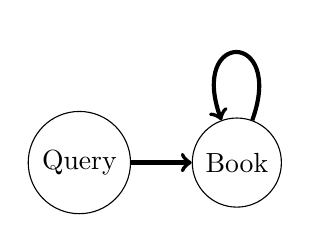
\begin{tikzpicture}
            \node[circle, draw] (n1) at (0,0) {Query};
            \node[circle, draw] (n2) at (2,0) {Book};

            \draw[->, line width=1.5pt] (n1) -- (n2);
            \draw[->, line width=1.5pt, looseness=8] (n2) to[out=70, in=110] (n2);
        \end{tikzpicture}
    \end{minipage}
    \caption{GraphQL-Schema als Graph}
    \label{schemgg}
\end{figure}

Generell starten alle GraphQL-Querys im Query-Type.
Erlaubte Anfragen sind dann alle Pfade, deren Ursprung im Query Knoten liegt, wobei Limitierungen implementiert werden können.
Property-based Testing nimmt die definierten Felder im Query-Type und geht die Pfade, welche sich im Graphen ergeben, zufällig ab.
Nach einer bestimmten Anzahl an zufälligen Iterationen wird die Query aus dem erlangten Pfad generiert und ausgeführt.
Wird jedoch ein wesentlich größeres Schema, zum Beispiel die GraphQL-API von GitLab~\cite{gitlab} genutzt, so erkennt man schnell, dass
der Graph so komplex wird, dass eine zufällige Pfadgenerierung zu unzuverlässig und ineffizient ist, um
eine große Struktur zuverlässig zu testen.
Einen ähnlichen Sachverhalt findet man in der Testgenerierung für Programmcode.
Dieser kann sehr komplex werden und es müssen Strategien gefunden werden, um diese effizient und zuverlässig zu testen.
Ein häufig verwendeter Ansatz ist es, den Code in einen Kontrollflussgraphen zu überführen, bei dem die Knoten Anweisungen oder Operationen darstellen
und die Kanten den möglichen Pfaden entsprechen, die während der Ausführung des Programms genommen werden können.
Hierbei wurde schon erhebliche Arbeit geleistet und diverse Kriterien entwickelt, wie man eine gute Testabdeckung erreicht.
An dieser Stelle sei insbesondere an \textit{Introduction to Software Testing}~\cite{software-testing} verwiesen.
In ~\cite{software-testing} wird die Graphenabdeckung erarbeitet und praktisch gezeigt, wie sie helfen kann, um Tests zu generieren.
Es werden verschiedene Kriterien vorgestellt, die den Graphen auf unterschiedliche Art und Weise betrachten.
Ziel ist es, zu zeigen, dass das in~\cite{software-testing} erarbeitete Wissen nicht nur für die Testentwicklung von Programmcode zielführend ist,
sondern auch für die Testgenerierung von anderen Graphstrukturen verwandt werden kann, in diesem Fall für die Testgenerierung für GraphQL-APIs.
Der Fokus wird sich auf die PrimePfad-Abdeckung~\cite[vgl. Criterion 2.4]{software-testing} richten, da zu vermuten ist, dass diese
Abdeckung einen guten Mittelweg zwischen Testgenauigkeit, Fehlerfindung und Effizienz bietet

\section{Umsetzung}

Zuallererst wird in dieser Arbeit die grundlegende Theorie in Kapitel~\ref{theorie} definiert und in Bezug zueinander gesetzt.
Es wird mit der Definition einiger Konzepte aus der Graphentheorie in Abschnitt~\ref{sec:graphentheorie} begonnen.
Darauffolgend kommt eine präzise Betrachtung von GraphQL in Absatz~\ref{graphql}.
Die Erkenntnisse beider Absätze werden dann in Absatz~\ref{graphtheorieQL} kombiniert.
Abschließend für die grundlegende Theorie wird in Absatz~\ref{test} das Thema Softwaretests eingeführt.
Die zuvor erarbeitete Theorie wird dann im Kapitel~\ref{gqlcov} genutzt, um einen Zugang zu schaffen, der zeigt, dass Graphabdeckungskriterien nutzbar für GraphQL sind.
Ein Überblick über den aktuellen Stand der Forschung wird in Kapitel~\ref{relatedWork} gegeben,
Darauffolgend wird mit dem gewonnenen Wissen in Kapitel~\ref{testentwurf} eine Methode entwickelt, die fähig ist, GraphQL automatisiert zu testen.
Die entwickelte Methode wird mit einem Prototypen verifiziert, wobei die Entwicklung von diesem in Kapitel~\ref{testautomatisierung} betrachtet wird.
Um die Fähigkeiten des Prototypen nachzuweisen, sind verschiedene Experimente in Kapitel~\ref{experimente} zu finden.
Ein Ausblick für zukünftige Weiterarbeit findet sich in Kapitel~\ref{futurework}.
Abschließen wird die Arbeit in Kapitel~\ref{fazit} mit einem Fazit, wo noch einmal die ganze Arbeit kurz rekapituliert wird.
